%%%%%%%%%%%%%%%%%%%%%%%%%%%%%%%%%%%%%%%%%%%%%%%%%%%%%%%%%%%%%%%%%%%%%%%%%%%%%%%
%Tutorial slides on Python.
%
% Author: FOSSEE
% Copyright (c) 2009, FOSSEE, IIT Bombay
%%%%%%%%%%%%%%%%%%%%%%%%%%%%%%%%%%%%%%%%%%%%%%%%%%%%%%%%%%%%%%%%%%%%%%%%%%%%%%%%

\documentclass[14pt,compress]{beamer}
%\documentclass[draft]{beamer}
%\documentclass[compress,handout]{beamer}
%\usepackage{pgfpages}
%\pgfpagesuselayout{2 on 1}[a4paper,border shrink=5mm]

% Modified from: generic-ornate-15min-45min.de.tex
\mode<presentation>
{
  \usetheme{Warsaw}
  \useoutertheme{infolines}
  \setbeamercovered{transparent}
}

\usepackage[english]{babel}
\usepackage[latin1]{inputenc}
%\usepackage{times}
\usepackage[T1]{fontenc}

% Taken from Fernando's slides.
\usepackage{ae,aecompl}
\usepackage{mathpazo,courier,euler}
\usepackage[scaled=.95]{helvet}

\definecolor{darkgreen}{rgb}{0,0.5,0}

\usepackage{listings}
\lstset{language=Python,
    basicstyle=\ttfamily\bfseries,
    commentstyle=\color{red}\itshape,
  stringstyle=\color{darkgreen},
  showstringspaces=false,
  keywordstyle=\color{blue}\bfseries}

%%%%%%%%%%%%%%%%%%%%%%%%%%%%%%%%%%%%%%%%%%%%%%%%%%%%%%%%%%%%%%%%%%%%%%
% Macros
\setbeamercolor{emphbar}{bg=blue!20, fg=black}
\newcommand{\emphbar}[1]
{\begin{beamercolorbox}[rounded=true]{emphbar}
      {#1}
 \end{beamercolorbox}
}
\newcounter{time}
\setcounter{time}{0}
\newcommand{\inctime}[1]{\addtocounter{time}{#1}{\tiny \thetime\ m}}

\newcommand{\typ}[1]{\lstinline{#1}}

\newcommand{\kwrd}[1]{ \texttt{\textbf{\color{blue}{#1}}}  }

\newcommand{\num}{\texttt{numpy}}

%%% This is from Fernando's setup.
% \usepackage{color}
% \definecolor{orange}{cmyk}{0,0.4,0.8,0.2}
% % Use and configure listings package for nicely formatted code
% \usepackage{listings}
% \lstset{
%    language=Python,
%    basicstyle=\small\ttfamily,
%    commentstyle=\ttfamily\color{blue},
%    stringstyle=\ttfamily\color{orange},
%    showstringspaces=false,
%    breaklines=true,
%    postbreak = \space\dots
% }


%%%%%%%%%%%%%%%%%%%%%%%%%%%%%%%%%%%%%%%%%%%%%%%%%%%%%%%%%%%%%%%%%%%%%%
% Title page
\title[Lists and Arrays]{Introductory Scientific Computing with
Python}
\subtitle{More plotting, lists and numpy arrays}

\author[FOSSEE] {FOSSEE}

\institute[FOSSEE -- IITB] {Department of Aerospace Engineering\\IIT Bombay}
\date[] {Mumbai, India}

%%%%%%%%%%%%%%%%%%%%%%%%%%%%%%%%%%%%%%%%%%%%%%%%%%%%%%%%%%%%%%%%%%%%%%

%\pgfdeclareimage[height=0.75cm]{iitmlogo}{iitmlogo}
%\logo{\pgfuseimage{iitmlogo}}


%% Delete this, if you do not want the table of contents to pop up at
%% the beginning of each subsection:
\AtBeginSubsection[]
{
  \begin{frame}<beamer>
    \frametitle{Outline}
    \tableofcontents[currentsection,currentsubsection]
  \end{frame}
}

\AtBeginSection[]
{
  \begin{frame}<beamer>
    \frametitle{Outline}
    \tableofcontents[currentsection,currentsubsection]
  \end{frame}
}

% If you wish to uncover everything in a step-wise fashion, uncomment
% the following command:
%\beamerdefaultoverlayspecification{<+->}

%\includeonlyframes{current,current1,current2,current3,current4,current5,current6}

%%%%%%%%%%%%%%%%%%%%%%%%%%%%%%%%%%%%%%%%%%%%%%%%%%%%%%%%%%%%%%%%%%%%%%
% DOCUMENT STARTS
\begin{document}

\begin{frame}
  \titlepage
\end{frame}

\begin{frame}
  \frametitle{Outline}
  \tableofcontents
  % You might wish to add the option [pausesections]
\end{frame}

\section{Plotting Points}
\begin{frame}[fragile]
\frametitle{Why would I plot f(x)?}
Do we plot analytical functions or experimental data?
\begin{small}
\begin{lstlisting}
In []: time = [0., 1., 2, 3]

In []: distance = [7., 11, 15, 19]

In []: plot(time,distance)
Out[]: [<matplotlib.lines.Line2D object at 0xa73aa8c>]

In []: xlabel('time')
Out[]: <matplotlib.text.Text object at 0x986e9ac>

In []: ylabel('distance')
Out[]: <matplotlib.text.Text object at 0x98746ec>
\end{lstlisting}
\end{small}
\end{frame}

\begin{frame}[fragile]
\begin{figure}
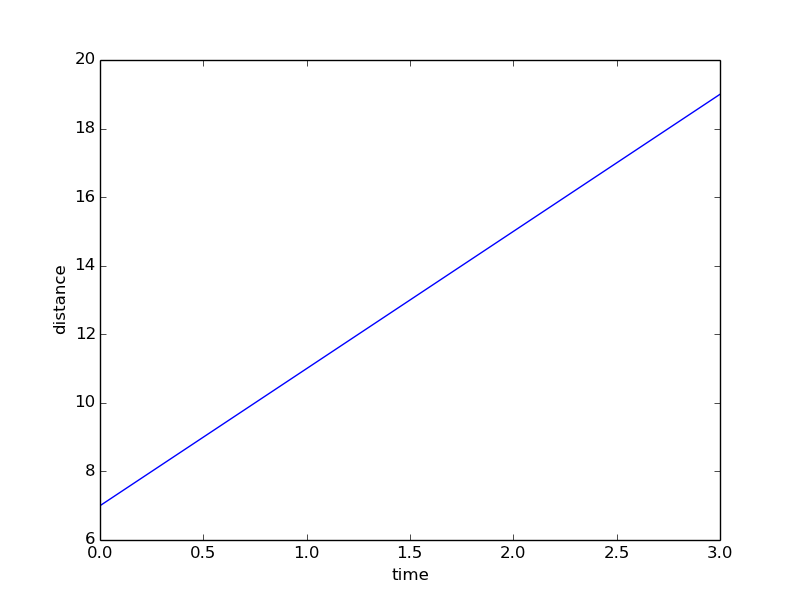
\includegraphics[width=3.5in]{data/straightline.png}
\end{figure}
\alert{Is this what you have?}
\end{frame}

\begin{frame}[fragile]
\frametitle{Plotting points}
\begin{itemize}
\item What if we want to plot the points?
\end{itemize}
\begin{lstlisting}
  In []: clf()

  In []: plot(time, distance, 'o')
  Out[]: [<matplotlib.lines.Line2D object at 0xac17e0c>]

  In []: clf()
  In []: plot(time, distance, '.')
  Out[]: [<matplotlib.lines.Line2D object at 0xac17e0c>]
\end{lstlisting}
\end{frame}

\begin{frame}[fragile]
\begin{figure}
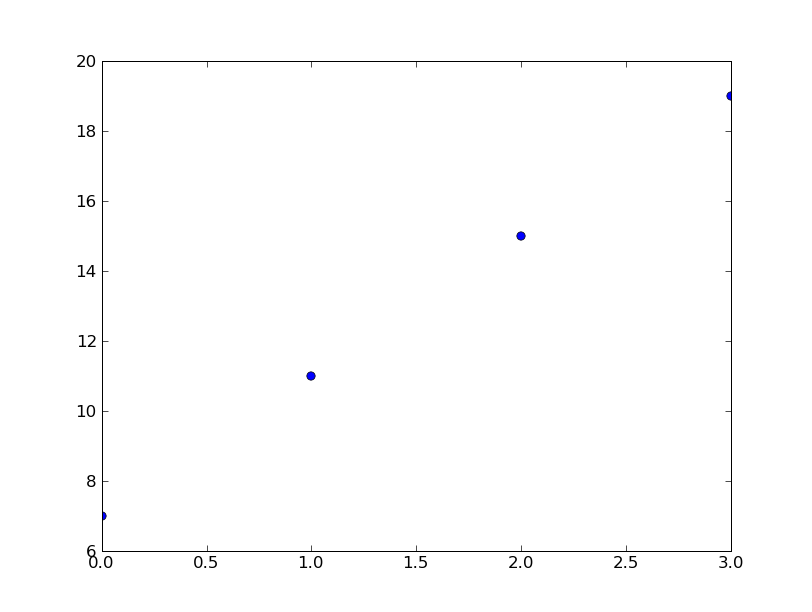
\includegraphics[interpolate=true,width=2.35in]{data/stline_dots.png}
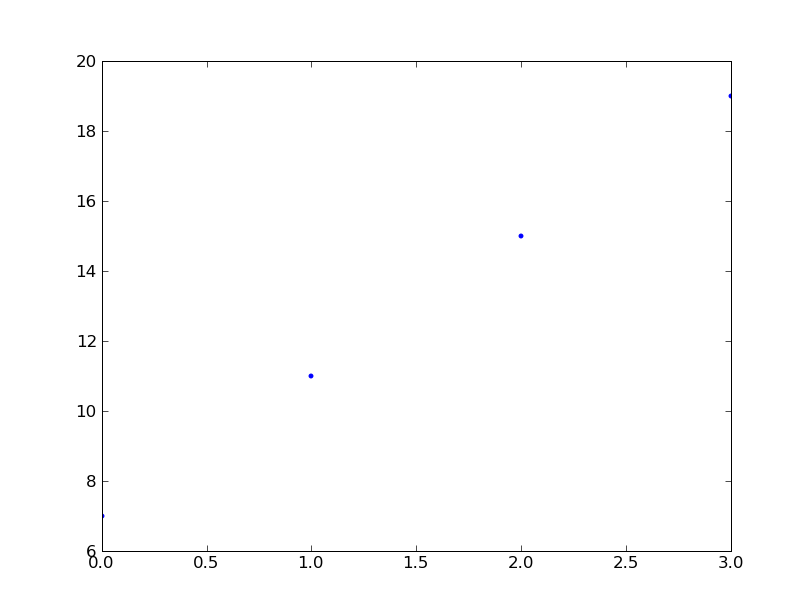
\includegraphics[interpolate=true,width=2.35in]{data/stline_points.png}
\end{figure}
\end{frame}

\begin{frame}[fragile]
\frametitle{Additional Line Styles}
\begin{itemize}
  \item \typ{'o'} - Filled circles
  \item \typ{'.'} - Small Dots
  \item \typ{'-'} - Lines
  \item \typ{'--'} - Dashed lines
\end{itemize}
\end{frame}

\section{Lists}
\begin{frame}[fragile]
  \frametitle{Lists: Introduction}
  \begin{lstlisting}
In []: time = [0., 1., 2, 3]

In []: distance = [7., 11, 15, 19]
  \end{lstlisting}
What are \typ{time} and \typ{distance}?\\
\begin{center}
  \large
\alert{\typ{lists!!}}
\end{center}
\end{frame}

\begin{frame}[fragile]
\frametitle{Lists: Initializing \& accessing elements}
\begin{lstlisting}
In []: mtlist = []
\end{lstlisting}
\emphbar{Empty List}
\begin{lstlisting}
In []: p = [ 2, 3, 5, 7]

In []: p[1]
Out[]: 3

In []: p[0]+p[1]+p[-1]
Out[]: 12
\end{lstlisting}
\end{frame}

\begin{frame}[fragile]
  \frametitle{List: Slicing}
  \begin{block}{Remember\ldots}
	\kwrd{In []: p = [ 2, 3, 5, 7]}
  \end{block}
\begin{lstlisting}
In []: p[1:3]
Out[]: [3, 5]
\end{lstlisting}
\emphbar{A slice}
\begin{lstlisting}
In []: p[0:-1]
Out[]: [2, 3, 5]
In []: p[1:]
Out[]: [3, 5, 7]
\end{lstlisting}
\end{frame}

\begin{frame}[plain,fragile]
  \frametitle{List: Slicing \ldots}
  \vspace*{-0.1in}
  \begin{small}
  \begin{block}{Remember\ldots}
	\kwrd{In []: p = [ 2, 3, 5, 7]}
\end{block}
\end{small}
\begin{lstlisting}
In []: p[0:4:2]
Out[]: [2, 5]
In []: p[0::2]
Out[]: [2, 5]
In []: p[::2]
Out[]: [2, 5]
In []: p[::3]
Out[]: [2, 7]
In []: p[::-1]
Out[]: [7, 5, 3, 2]
\end{lstlisting}
\alert{\typ{list[initial:final:step]}}
\end{frame}

\begin{frame}[fragile]
  \frametitle{List: Slicing}
  \begin{block}{Remember\ldots}
	\kwrd{In []: p = [ 2, 3, 5, 7]}
  \end{block}
  What is the output of the following?
\begin{lstlisting}
In []: p[1::2]

In []: p[1:-1:2]
\end{lstlisting}
\end{frame}


%% more on list slicing
\begin{frame}[fragile]
\frametitle{List operations}
\begin{lstlisting}
In []: b = [ 11, 13, 17]
In []: c = p + b

In []: c
Out[]: [2, 3, 5, 7, 11, 13, 17]

In []: p.append(11)
In []: p
Out[]: [ 2, 3, 5, 7, 11]
\end{lstlisting}
Question: Does \typ{c} change now that \typ{p} is changed?
\inctime{10}
\end{frame}

\section{Simple Pendulum}
\begin{frame}[fragile]
\frametitle{Simple Pendulum - L and T}
Let us look at the Simple Pendulum experiment.
\begin{center}
\begin{small}
\begin{tabular}{| c | c | c |}
\hline
$L$ & $T$ & $T^2$ \\ \hline
0.2 & 0.90 & \\ \hline
0.3 & 1.19 & \\ \hline
0.4 & 1.30 & \\ \hline
0.5 & 1.47 & \\ \hline
0.6 & 1.58 & \\ \hline
0.7 & 1.77 & \\ \hline
0.8 & 1.83 & \\ \hline
\end{tabular}
\end{small}\\
\alert{$L \alpha T^2$}
\end{center}
\end{frame}

\begin{frame}[fragile]
\frametitle{Lets use lists}
\begin{lstlisting}
In []: L = [0.2, 0.3, 0.4, 0.5,
            0.6, 0.7, 0.8]

In []: t = [0.90, 1.19, 1.30,
            1.47, 1.58, 1.77,
            1.83]
\end{lstlisting}
\alert{Gotcha}: Make sure \typ{L} and \typ{t} have the same number
of elements

\begin{lstlisting}
In []: print(len(L), len(t))
\end{lstlisting}

\end{frame}

\begin{frame}[fragile]
\frametitle{Plotting $L$ vs $T^2$}
\begin{itemize}
\item We must square each of the values in \typ{t}
\item How do we do it?
\item We use a \kwrd{for} loop to iterate over \typ{t}
\end{itemize}
\end{frame}

\begin{frame}[fragile]
\frametitle{Looping with \texttt{for}}
\begin{lstlisting}
In []: for time in t:
 ....:     print(time*time)
 ....:
 ....:
\end{lstlisting}
This will print the square of each item in the list, \typ{t}
\end{frame}

\begin{frame}[fragile]
\frametitle{Plotting $L$ vs $T^2$}
\begin{lstlisting}
In []: tsq = []

In []: for time in t:
 ....:     tsq.append(time*time)
 ....:
 ....:

\end{lstlisting}
This gives \typ{tsq} which is the list of squares of \typ{t} values.
\begin{lstlisting}
In []: print(len(L), len(t), len(tsq))
Out[]: (7, 7, 7)

In []: plot(L, tsq)
\end{lstlisting}
\end{frame}

\begin{frame}[fragile]
\begin{figure}
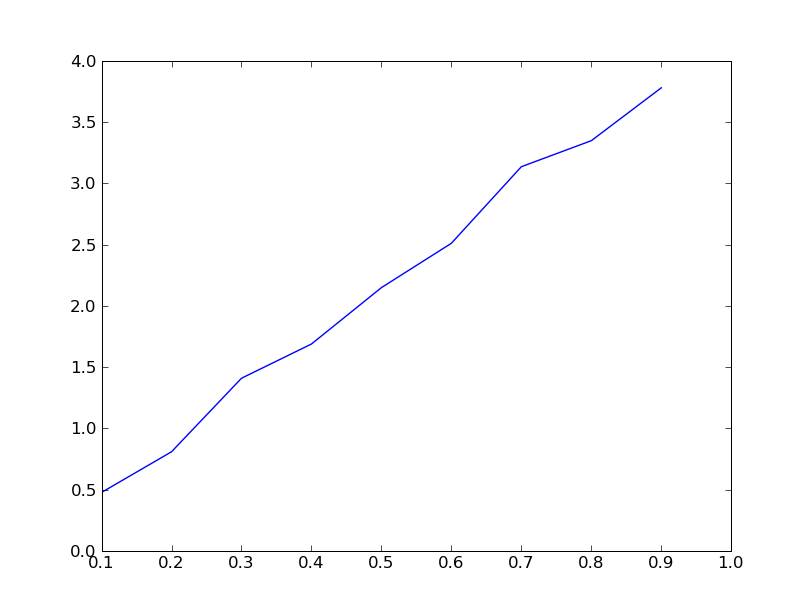
\includegraphics[width=3.5in]{data/L-TSq-limited.png}
\end{figure}
\inctime{10}
\end{frame}


\begin{frame}[fragile]
\frametitle{Don't repeat yourself: functions}
\noindent Let us define a function to square the list
\begin{lstlisting}
In []: def sqr(arr):
  ...:     result = []
  ...:     for x in arr:
  ...:         result.append(x*x)
  ...:     return result
  ...:

In []: tsq = sqr(t)

\end{lstlisting}  %$
\end{frame}

\begin{frame}[fragile]
  \frametitle{More on defining functions}
  \begin{itemize}
  \item Consider the function \texttt{f(x) = x\textasciicircum{}2}
  \item Let's write a Python function, equivalent to this
  \end{itemize}
  \begin{lstlisting}
   In[]: def f(x):
   ....:     return x*x
   ....:

   In[]: f(1)
   In[]: f(2)
  \end{lstlisting}
  \begin{itemize}
  \item \texttt{def} is a keyword
  \item \texttt{f} is the name of the function
  \item \texttt{x} the parameter of the function (local variable)
  \item \texttt{return} is a keyword
  \end{itemize}
\end{frame}

\begin{frame}[fragile]
  \frametitle{Aside: Exercise}
  \begin{itemize}
  \item Write a function called \typ{mysum(a, b)} that returns sum of two
    arguments.
  \end{itemize}
  \pause
\begin{lstlisting}
In []: def mysum(a, b):
  ...:    return a + b
  ...:
In []: mysum(1, 2)

In []: mysum([1, 2], [3, 4])
\end{lstlisting}
\end{frame}

\begin{frame}[fragile]
  \frametitle{This seems tedious}

  \begin{itemize}
  \item Do we have to write a function just to get the square of a list?
    \item Lists
\begin{itemize}
    \item Nice
    \item Not too convenient for math
    \item Slow
\end{itemize}
\item Enter NumPy arrays
    \begin{itemize}
        \item Fixed size, data type
        \item Very convenient
        \item Fast
    \end{itemize}
  \end{itemize}
  \inctime{10}
\end{frame}

\subsection{\num\ arrays}

\begin{frame}[fragile]
\frametitle{NumPy arrays}
\begin{lstlisting}
In []: t = array(t)

In []: tsq = t*t

In []: print(tsq)

In []: plot(L, tsq) # works!
\end{lstlisting}  %$
\end{frame}

\begin{frame}[fragile]
\frametitle{Speed?}

\noindent Lets use range to create a large list.

\begin{lstlisting}
In []: t = range(1000000)

In []: tsq = sqr(t)

\end{lstlisting}  %$

\noindent Now try it with

\begin{lstlisting}
In []: t = array(t)

In []: tsq = t*t
\end{lstlisting}
\ldots
\end{frame}


\begin{frame}[fragile]
  \frametitle{IPython tip: Timing}

Try the following:
  \begin{lstlisting}
In []: %timeit sqr(t)

In []: %timeit?

  \end{lstlisting}

  \begin{itemize}
      \item \typ{\%timeit}: accurate, many measurements
      \item Can also use \typ{\%time}
      \item \typ{\%time}: less accurate, one measurement
  \end{itemize}

\inctime{10}
\end{frame}


\begin{frame}[fragile]
\frametitle{Exercise}
\begin{center}
    Find out the speed difference between the \typ{sqr} function and
    \typ{t*t} on the numpy array.
\end{center}

\end{frame}

\begin{frame}[fragile]
  \frametitle{Solution}
\begin{lstlisting}
In []: t = linspace(0, 10, 100000)
In []: %timeit sqr(t)
In []: %timeit t*t
\end{lstlisting}
  \inctime{5}
\end{frame}

\begin{frame}[fragile]
\frametitle{Summary}
\begin{itemize}
\item Plot attributes
\item plotting points
\item Lists
\item Defining simple functions
\item Introduction to \num\ arrays
\item Timing with \typ{\%timeit}
\end{itemize}
\end{frame}

\end{document}
